\documentclass[11pt]{article}

\usepackage{amsmath}
\usepackage{amsfonts}
\usepackage[margin=1in]{geometry}
\usepackage{enumitem}
\usepackage{graphicx}
\usepackage[colorlinks]{hyperref}

\usepackage{longtable}

\usepackage{helvet}
\renewcommand{\familydefault}{\sfdefault}

\setlength{\parindent}{0in}

\def\tightlist{}
\def\toprule{}
\def\bottomrule{}

\begin{document}

Preface: Homework in this class is a very large part of the learning
experience (and a large fraction of your grade!). The homework might
look long, but that is because it not really serving as a check on
whether you are getting things from lecture. It meant to help you learn
the material, the importance of different aspects of the material, and
the implications of the material on your future work. So there will
typically be longer descriptions in the problem statements. The work you
are being asked to do is no longer than a standard lecture course, but
the kinds of questions might be different. We strongly encourage you to
work together (and with Dennis and Danny) on these homework problems,
but you must turn in your own work.

\section{Homework 1 (Due September
9th)}\label{homework-1-due-september-9th}

Homework 1 emphasizes the mathematical formalism and related thinking
that you will draw on in class. This homework focuses on Sections
1.1-1.4 of Griffiths, which covers differential, integral, and vector
calculus. It also serves as an introduction to using
\href{http://jupyter.org}{Jupyter notebooks}, which you will use on most
homework assignments. With regard to computation on this homework, you
will be using the \href{http://sympy.org}{sympy} library, which allows
you to perform symbolic manipulations (like Mathematica), and the
\href{http://matplotlib.org/}{matplotlib} library, which allows you to
plot different kinds of figures.

\paragraph{1. Reminders of Integrals
Past}\label{reminders-of-integrals-past}

In this course, you will perform lots of different kinds of integrals,
some of which you might have done in previous courses. In this problem,
we will just dust off some of those integration techniques. You will
need to explain key steps of the integration for each one, not simply do
the mathematics.

\begin{enumerate}
\def\labelenumi{\arabic{enumi}.}
\tightlist
\item
  Line (or path) integrals - These integrals are important for thinking
  about energy. Determine the work done by the vector force
  \(\mathbf{F} = y^2\;\hat{x} - 2x^2\;\hat{y}\) along the parabolic path
  \(y=x^2\) from (0,0) to (2,4). This path is restricted to the x-y
  plane and recall that \(W=\int \mathbf{F}\cdot d\mathbf{l}\).
\item
  Surface integrals - Calculating the flux over a particular surface is
  a very common way of determine the electric field. Evaluate the
  integral \(\int_S \mathbf{v}\cdot d\mathbf{A}\) where
  \(\mathbf{v}(x,y,z) = 2x\;\hat{y} + 2y\;\hat{z}\) and \(S\) is the
  rectangular surface lying in x-y plane from (0,0) to (1,5). Choose the
  direction of \(+\hat{z}\) to be indicative of positive flux.
\item
  Volume integrals - It will be common for you to determine the amount
  of total charge in a situation where the charge is distributed in
  space according to some function. You might be familiar with this
  concept from the perspective of distributed mass. Consider two
  different spheres: one with uniform mass density, \(\rho_0\), and the
  other with a radially varying density,
  \(\rho(r)=\frac{3\rho_0}{2R^2}r^2\). If both spheres have the same
  radius \(R\), which has more mass?
\end{enumerate}

\paragraph{2. What can be done to a scalar
function?}\label{what-can-be-done-to-a-scalar-function}

Given the scalar function \(T(x,y,z)\) (e.g., the temperature at any
point in the room), which of the three operations (div, grad, and/or
curl) can be sensibly operated on \(T\)? For each which can:

\begin{enumerate}
\def\labelenumi{\arabic{enumi}.}
\tightlist
\item
  give a formula for the result,
\item
  explain in words how you would interpret the result, and
\item
  identify if the result a vector or scalar.
\end{enumerate}

\paragraph{3. What can be done to a vector
function?}\label{what-can-be-done-to-a-vector-function}

Given the vector function \(\vec{V}(x,y,z)\) (e.g., the velocity of a
flowing fluid), which of the three operations (div, grad, and/or curl)
can be sensibly operated on \(\vec{V}\)? For each which can:

\begin{enumerate}
\def\labelenumi{\arabic{enumi}.}
\tightlist
\item
  give a formula for the result,
\item
  explain in words how you would interpret the result, and
\item
  identify if the result a vector or scalar.
\end{enumerate}

\paragraph{4. Determine the gradient of a scalar function and check it
with computational
tools}\label{determine-the-gradient-of-a-scalar-function-and-check-it-with-computational-tools}

In Griffiths, \(\vec{\mathfrak{r}}\) represents the separation vector
between source charges \(\langle x', y', z' \rangle\) and the field
point -- location of test charge -- \(\langle x, y, z \rangle\). The
separation vector is a \textbf{critically important} vector in
electrodynamics as it underlies all of the mathematical models that
describe how source charges produce electric and magnetic fields. To
that end, you will often do some mathematical manipulations of the
separation vector. You are asked to perform two common manipulations
below.

\begin{enumerate}
\def\labelenumi{\arabic{enumi}.}
\tightlist
\item
  Calculate the gradient of the magnitude of the separation vector
  (i.e., \(\nabla\|\vec{\mathfrak{r}}\|\)) and the gradient of the
  inverse of the magnitude of the separation vector (i.e.,
  \(\nabla \dfrac{1}{\|\vec{\mathfrak{r}}\|}\)) and show the gradients
  of these functions can be written as functions of the separation
  vector (\(\vec{\mathfrak{r}}\)) and/or its magntiude
  (\(\|\vec{\mathfrak{r}}\|\)). (\emph{Hint: it might be easier to do
  this by explicitly writing out the function in Cartesian
  coordinates.})
\item
  After determining the gradients of each of these functions by hand,
  \href{../jupyter/HW1-GradientProblem.ipynb}{download this Jupyter
  notebook} (you can
  \href{https://github.com/dannycab/phy481msu/blob/gh-pages/jupyter/HW1-GradientProblem.ipynb}{view
  it here}), which demonstrates how to calculate gradients using the
  \href{http://sympy.org}{sympy} library for Python. Working through the
  notebook, use it to check the work you did by hand. Do you get the
  same answers?
\end{enumerate}

\textbf{Important: In this class, we are strongly encouraging you to use
the tools of modern science (i.e., computing) in a responsible way. This
problem demonstrates that you may want to use Python and sympy to check
the work that you have done analytically.}

\paragraph{5. Analyzing divergence and curl
visually}\label{analyzing-divergence-and-curl-visually}

Calculating the divergence and curl of a vector field analytically is
possible when the field is a well-known function (e.g.,
\(\vec{V}(x,y,z)\)). However, it will not always be the case that you
know the function that generates the vector field. For example, in
experimental fluid mechanics, measurements of the velocity field are
done by tracking individual particles (called ``tracers'') that move in
the field.

\href{https://www.youtube.com/watch?v=hzvFHrWQbP0}{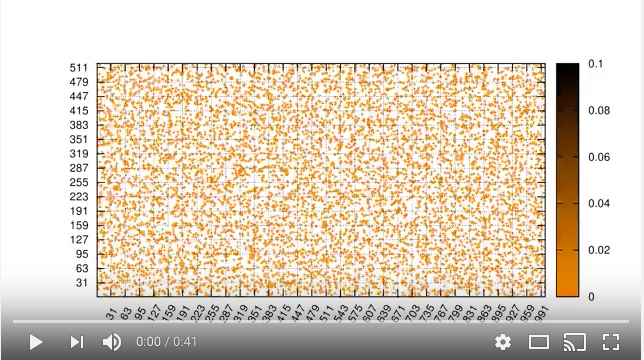
\includegraphics[width=0.6\linewidth]{./images/hw1/tracers.png}}

The displacement of those tracers is used to numerically reconstruct the
velocity field of the fluid (by way of numerical derivatives), which
usually does not conform to a known function. However, it is important
to know if the flow has divergence or curl overall or at specific points
as the models for fluid flow that are used to analyze the velocity field
strongly depend on these results. Hence, visual inspection of a field
(in our case, electromagnetic fields) is an important tool to understand
which models might be used to analyze the field. This will be
exceedingly important in our distinction between electric and magnetic
fields as well as when the fields begin to vary with time.

For each of the four vector fields sketched below:

\begin{enumerate}
\def\labelenumi{\arabic{enumi}.}
\tightlist
\item
  Which of them have a nonzero \emph{divergence} somewhere? (If the
  divergence is nonzero \emph{only} at isolated points, which point(s)
  would that be?)
\item
  Which of the following fields have nonzero \emph{curl} somewhere? (If
  the curl is nonzero \emph{only} at isolated points, which point(s)
  would that be?)
\item
  Provide a brief explanation for each of your answers above.
\end{enumerate}

\begin{longtable}[]{@{}cc@{}}
\toprule
Field A & Field B\tabularnewline
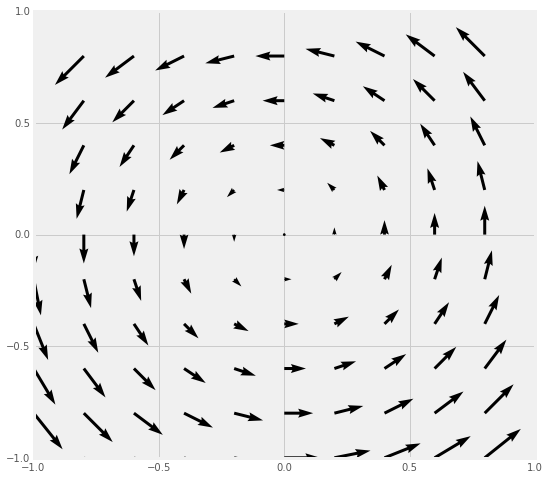
\includegraphics[width=0.4\linewidth]{./images/hw1/A.png} &
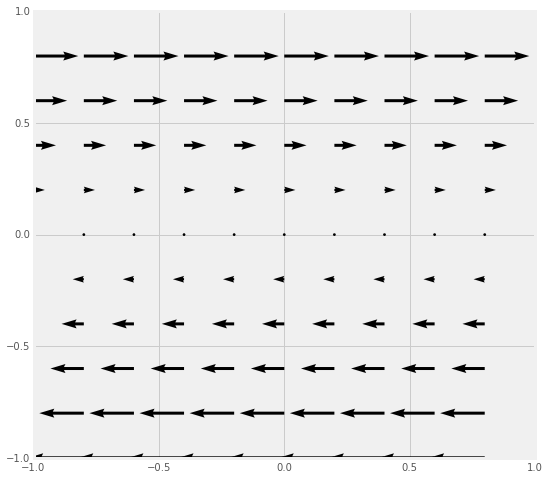
\includegraphics[width=0.4\linewidth]{./images/hw1/B.png}\tabularnewline
Field C & Field D\tabularnewline
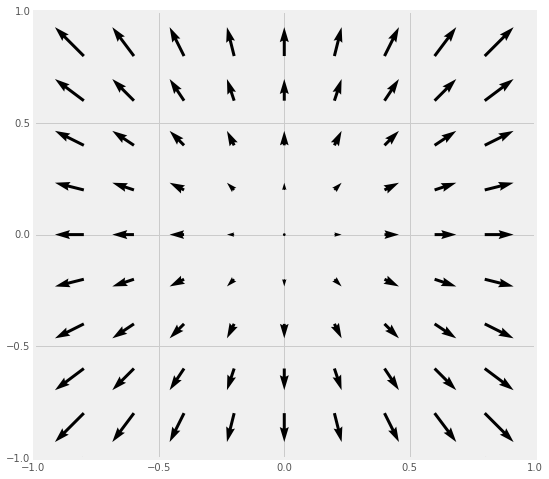
\includegraphics[width=0.4\linewidth]{./images/hw1/C.png} &
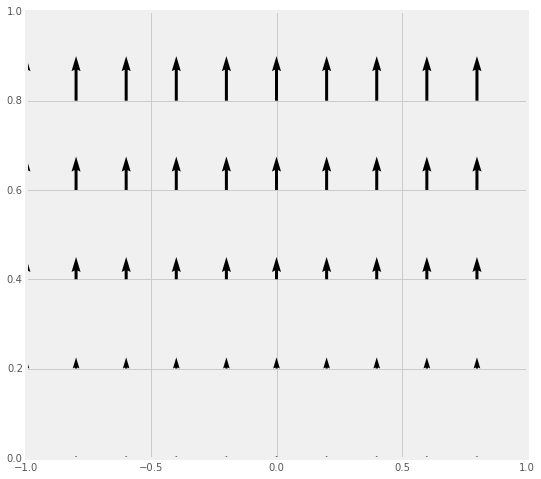
\includegraphics[width=0.4\linewidth]{./images/hw1/D.png}\tabularnewline
\bottomrule
\end{longtable}

\paragraph{\texorpdfstring{6. Plotting vector functions with
\texttt{matplotlib}}{6. Plotting vector functions with matplotlib}}\label{plotting-vector-functions-with-matplotlib}

Physics is both a mathematical and visual science. It is important to
develop the ability to sketch and plot figures of various types. For the
early part of this class, plotting the field generated by electric
charges is important to understanding the field itself. In this problem,
you will learn to use the
\href{http://matplotlib.org}{\texttt{matplotlib} library} to
\href{http://matplotlib.org/examples/pylab_examples/quiver_demo.html}{plot
vector fields}. As with the previous computational problem, you can
\href{../jupyter/HW1-VectorFieldsProblem.ipynb}{download this working
Jupyter notebook}
(\href{https://github.com/dannycab/phy481msu/blob/gh-pages/jupyter/HW1-VectorFieldsProblem.ipynb}{view
it here}), which describes how this kind of plotting is done for a
specific case (\(\vec{v}(x,y)=y\hat{x}\)).

It will be up to you to plot additional figures for these cases:

\begin{enumerate}
\def\labelenumi{\arabic{enumi}.}
\tightlist
\item
  \(\vec{v}(x,y)=r\hat{r}\) (where \(\vec{r}\) refers to the usual
  \(\vec{r}\) in spherical coordinates.)
\item
  \(\vec{v}(x,y) = \dfrac{x}{(\sqrt{x^2+y^2})^3}\hat{x}+\dfrac{y}{(\sqrt{x^2+y^2})^3}\hat{x}\)
\item
  \(\vec{v}(x,y) = \hat{\phi}\) (where \(\\phi\) is the usual
  plane-polar coordinate.)
\item
  For each case above, can you describe a physical situation where the
  field would be applicable?
\end{enumerate}

\paragraph{7. Vector proofs can be incredibly
useful}\label{vector-proofs-can-be-incredibly-useful}

In electromagnetism, developing a deep understanding of vector
mathematics can facilitate a deeper understanding of the physical
systems that we will investigate. While we will rarely ask you to prove
relationships outright, knowing how certain proofs are done can often
help you simplify a complicated problem. For example, in this problem,
you will learn how we often use general vector operations with
unspecified surfaces to make general statements about the field. In
Griffiths, you read about a few integral theorems: the gradient theorem,
Gauss's theorem (for divergences), and Stokes' theorem (for curls). You
will make use of those theorems to prove a few things you have some
intuition about from vector calculus.

\begin{enumerate}
\def\labelenumi{\arabic{enumi}.}
\tightlist
\item
  From vector calculus, you know that the curl of any gradient of any
  scalar field is zero: $\nabla \times \nabla T(x,y,z) = 0 $. Use the
  corollary of the gradient theorem, namely that closed loop integral of
  any gradient of a scalar field is zero,
  \(\oint \nabla T\cdot d\mathbf{l} = 0\), along with Stokes' theorem,
  \(\int_S(\nabla \times \mathbf{v})\cdot d\mathbf{a} = \oint_C \mathbf{v}\cdot d\mathbf{l}\),
  to demonstrate that the curl of a gradient is zero. What is the
  essential argument that needs to be made that proves that the result
  is generalizable to any situation? (\emph{Hint: The surface (S) and
  thus the line (C) that bounds the surface are not specified.})
\item
  What does your result from the previous question tell you about
  possibility of swirly-ness of the gradient of a temperature field,
  \(\nabla T\), over any specified surface?
\item
  From vector calculus, you know that the divergence of the curl of any
  vector field is zero, \(\nabla \cdot (\nabla \times \mathbf{v}) = 0\).
  Use the corollary of Stokes' theorem, namely that the closed surface
  integral of the curl of a vector field is zero, $\oint\_S
  (\nabla \times \mathbf{v})\cdot d\mathbf{a} = 0 $, along with the
  divergence theorem,
  \(\int(\nabla \cdot \mathbf{v}) d\tau = \oint_S \mathbf{v}\cdot d\mathbf{a}\),
  to demonstrate that the divergence of a curl is zero. What is the
  essential argument that needs to be made the proves the result is
  generalizable to any situation? (\emph{Hint: The volume (V) and thus
  the surface (S) that bounds it are not specified.})
\item
  By doing these two proofs, what do you feel like you learned about
  vector calculus that you didn't already know?
\end{enumerate}

\end{document}
